\documentclass[12pt]{article}

\usepackage{fancyhdr}
\usepackage{extramarks}
\usepackage{amsmath}
\usepackage{amsthm}
\usepackage{amssymb}
\usepackage{amsfonts}
\usepackage{tikz}
\usepackage[plain]{algorithm}
\usepackage{algpseudocode}
\usepackage{graphicx}

\usetikzlibrary{automata,positioning}

%
% Basic Document Settings
%

\topmargin=-0.45in
\evensidemargin=0in
\oddsidemargin=0in
\textwidth=6.5in
\textheight=9.0in
\headsep=0.25in

\linespread{1.1}

\pagestyle{fancy}
\lhead{\hmwkAuthorName}
\chead{\hmwkClass\ \hmwkTitle}
\rhead{\firstxmark}
\lfoot{\lastxmark}
\cfoot{\thepage}

\renewcommand\headrulewidth{0.4pt}
\renewcommand\footrulewidth{0.4pt}

\setlength\parindent{0pt}

%
% Create Problem Sections
%

\newcommand{\enterProblemHeader}[1]{
    \nobreak\extramarks{}{Problem \arabic{#1} continued on next page\ldots}\nobreak{}
    \nobreak\extramarks{Problem \arabic{#1} (continued)}{Problem \arabic{#1} continued on next page\ldots}\nobreak{}
}

\newcommand{\exitProblemHeader}[1]{
    \nobreak\extramarks{Problem \arabic{#1} (continued)}{Problem \arabic{#1} continued on next page\ldots}\nobreak{}
    \stepcounter{#1}
    \nobreak\extramarks{Problem \arabic{#1}}{}\nobreak{}
}

\setcounter{secnumdepth}{0}
\newcounter{partCounter}
\newcounter{homeworkProblemCounter}
\setcounter{homeworkProblemCounter}{1}
\nobreak\extramarks{Problem \arabic{homeworkProblemCounter}}{}\nobreak{}

%
% Homework Problem Environment
%
% This environment takes an optional argument. When given, it will adjust the
% problem counter. This is useful for when the problems given for your
% assignment aren't sequential. See the last 3 problems of this template for an
% example.
%
\newenvironment{homeworkProblem}[1][-1]{
    \ifnum#1>0
        \setcounter{homeworkProblemCounter}{#1}
    \fi
    \section{Problem \arabic{homeworkProblemCounter}}
    \setcounter{partCounter}{1}
    \enterProblemHeader{homeworkProblemCounter}
}{
    \exitProblemHeader{homeworkProblemCounter}
}

%
% Homework Details
%   - Title
%   - Date
%   - Class
%   - Instructor
%   - Author
%

\newcommand{\hmwkTitle}{Homework\ \#5}
\newcommand{\hmwkDate}{2017-03-25}
\newcommand{\hmwkClass}{MATH6222}
\newcommand{\hmwkClassInstructor}{Instructor: Dr. David Smyth}
\newcommand{\hmwkTutor}{Tutor: Mark Bugden (Wednesday 1-2pm)}
\newcommand{\hmwkAuthorName}{\textbf{Rui Qiu u6139152}}

%
% Title Page
%

\title{
    \vspace{2in}
    \textmd{\textbf{\hmwkClass:\ \hmwkTitle}}\\
    \normalsize\vspace{0.1in}\small{\hmwkDate}\\
    \vspace{0.1in}\large{\textit{\hmwkClassInstructor}}\\
    \vspace{0.1in}
    	\large{\textit{\hmwkTutor}}
    \vspace{3in}
}

\author{\hmwkAuthorName}
\date{}

\renewcommand{\part}[1]{\textbf{\large Part \Alph{partCounter}}\stepcounter{partCounter}\\}

%
% Various Helper Commands
%

% New QED symbol
\renewcommand{\qedsymbol}{$\blacksquare$}

% Useful for algorithms
\newcommand{\alg}[1]{\textsc{\bfseries \footnotesize #1}}

% For derivatives
\newcommand{\deriv}[1]{\frac{\mathrm{d}}{\mathrm{d}x} (#1)}

% For partial derivatives
\newcommand{\pderiv}[2]{\frac{\partial}{\partial #1} (#2)}

% Integral dx
\newcommand{\dx}{\mathrm{d}x}

% Alias for the Solution section header
\newcommand{\solution}{\textbf{\large Solution}}

% Probability commands: Expectation, Variance, Covariance, Bias
\newcommand{\E}{\mathrm{E}}
\newcommand{\Var}{\mathrm{Var}}
\newcommand{\Cov}{\mathrm{Cov}}
\newcommand{\Bias}{\mathrm{Bias}}

\begin{document}

\maketitle

\pagebreak

\begin{homeworkProblem}
The summation identity for binomial coefficients states that:

\[\sum\limits^n_{i=0}{i \choose k} = {n+1 \choose k+1}\]

Give two proofs of this identity, one using the bug-path model for binomial coefficients, and one using induction.\\

\textbf{Proof 1:}\\

Since ${i \choose k} = 0$ if $i < k$. The left hand side (LHS) of this equation is equivalent to

\[\sum\limits^n_{i=0}{i \choose k} = {k \choose k} + {k + 1 \choose k} +\dots + {n \choose k}\]\\

What does it mean? By our bug-path model, each ${i \choose k}$ means the number of legit paths that a bug can take from point $(0,0)$ to point $(i-k, k)$.\\

(\textit{Note:} This is also equivalent to the number of legit paths that a bug can take from point $(0,0)$ to point $(k, i-k)$. But for simplicity, we take the first definition and stick to it.)\\

Therefore, the LHS stands for the total number of legit paths from $(0,0)$ to $(0,k), (1,k),\dots, (n-k,k)$.\\

Then what about the right hand side (RHS)? The right hand side stands for the number of legit paths from $(0,0)$ to $(n-k,k+1)$. The endpoint has the same x-coordinate as $(n-k,k)$ but one unit higher than that. Now consider how many such paths are there? Actually we can start from all the endpoints in our LHS, i.e. $(0, k), (1, k)\dots, (n-k,k)$. And if we start from any of those point, and we don't want to overlap any other paths, there is only one way to our target: \textbf{go up one unit, then go right till hitting the target.}\\

\begin{figure*}
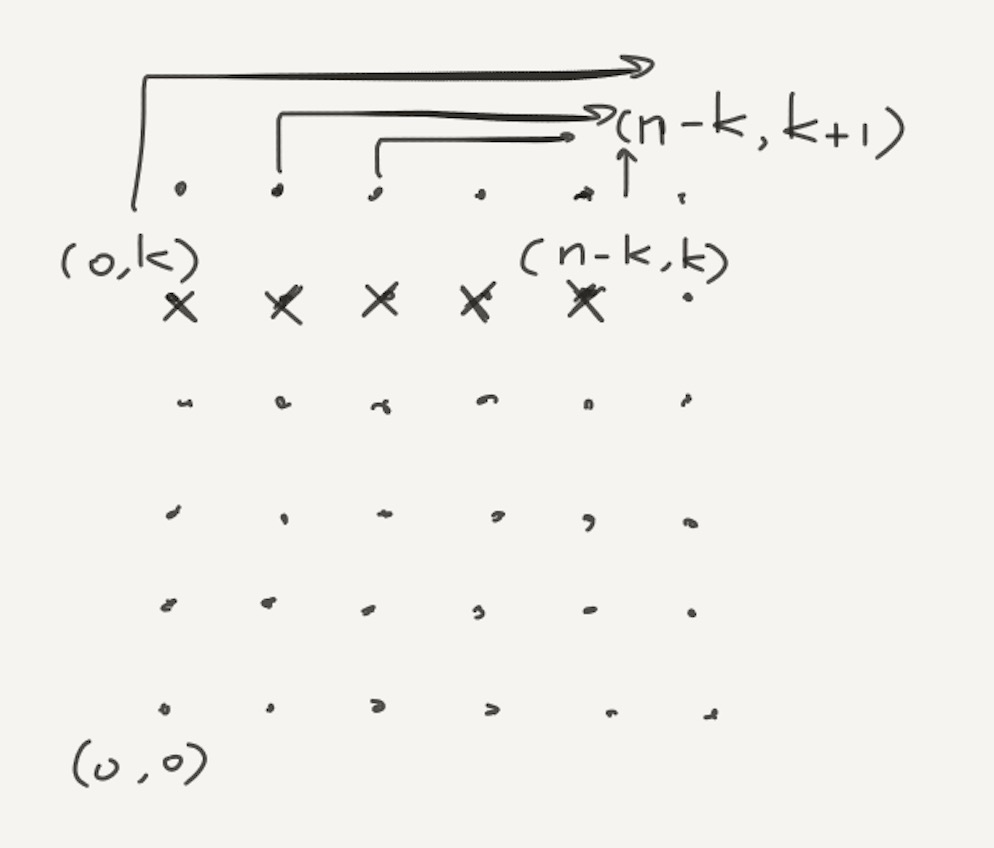
\includegraphics[scale=0.2]{images/bugpath.jpg}
\centering
\caption{Bug-path}
\end{figure*}

And we consider the possibility if there is a path from $(0,0)$ to $(n-k, k+1)$ that does not go through any of those points. The answer is no, because those points form "ceiling" from $x=0$ to $x=k$, and there is no way to go beyond $x=k$ and turn back. In other words, if a bug wants to go to $(n-k, k+1)$ as its destination, it has to go through those points.\\

Hence, there are ${k \choose k}$ ways from $(0,0)$ to $(0,k)$, $1$ way (no overlapping) from $(0,k)$ to $(n-k, k+1)$. Similarly, there are ${k+1 \choose k}$ ways from $(0,0)$ to $(1,k)$, $1$ way (no overlapping) from $(1,k)$ to $(n-k, k+1)$, etc. We sum them up and get LHS. And by definition it is our RHS. Therefore LHS=RHS.\\

\textbf{Proof 2:}\\

Let $P(n)$ be the statement that the equation holds for $n\in\mathbb{N}$.\\

\textbf{Base case $P(0)$}: Let $n=0$,

\begin{itemize}
	\item If $k=0$, then LHS=RHS=$1$.
	\item If $k>0$, then LHS=RHS=$0$.
\end{itemize}

So $P(n)$ is true.\\

\textbf{Inductive hypothesis:} Suppose $P(n-1)$ is true, i.e.

\[\sum\limits^{n-1}_{i=0}{i\choose k} = {n \choose k+1}\]\\

\textbf{Inductive step $P(n)$:}

\[
\begin{split}
	\sum\limits^n_{i=1}{i \choose k} &= \sum\limits^{n-1}_{i=0}{i \choose k} + {n \choose k}\\
	&={n\choose k+1}{n\choose k}\\
	&={n+1 \choose k+1} \ \ \ \ \ \ \ \ \ \ \text{(applied Pascal's formula here)}\\
\end{split}
\]
\qed 
\end{homeworkProblem}

\begin{homeworkProblem}
Give short, insightful proofs of the following formulae:\\

(a) ${n\choose k}{k\choose j} = {n\choose j}{n-j \choose k-j}.$\\

\textbf{Proof:}\\

Consider a scenario that Ash has $n$ Pok\'emons and he needs to select $k$ out of them in the battle, and due to limitations he can only give $j$ in-battle Pok\'emons berries (each Pok\'emon can only carry one berry). And now we want to find out how many different strategies he could have to arrange his Pok\'emon battle participation and berry arragements.\\

The left hand side can be interpreted as:
\begin{itemize}
	\item First there are ${n\choose k}$ ways to select $k$ Pok\'emons out of $n$.
	\item Then for $k$ selected Pok\'emons, there are ${k\choose j}$ ways to give them berries.
\end{itemize}

Then there are in total ${n\choose k}{k\choose j}$ ways.\\

The right hand side can be interpreted as:
\begin{itemize}
	\item First select $j$ Pok\'emons out of $n$, give them berries.
	\item Then for $n-j$ rest of Pok\'emons, we have to select $k-j$ number of Pok\'emons to make the total number of Pok\'emons in battle $k$. 
\end{itemize}

Then there are in total ${n\choose j}{n-j \choose k-j}$ ways.\\

(b) $\sum\limits^n_{k=0}k{n\choose k} = n 2^{n-1}.$\\

\textbf{Proof:}\\

Imagine a game with non-limited $k$ number of starting lineup players. We need to select $k$ players from total $n$ players. And the starting lineup also needs a team captain. So how many possible lineups can we select?\\

Left hand side: select a starting lineup of $k$ players from $n$ qualified players (${n\choose k}$ ways), then we select a team captain from $k$ people (${k\choose 1}=k$ ways). Also $k$ is uncertain, so we can sum them up, and generate the formula on LHS.\\

Right hand side: select a team captain from $n$ players first, then we divide the rest $n-1$ players to two groups: one in the starting lineup (non-captain), and the other out of lineup. There are $2^{n-1}$ ways to divide. So in total $n\cdot 2^{n-1}$ ways, which is just the formula on RHS.\\
\qed

\end{homeworkProblem}

\begin{homeworkProblem}
Count the sets of six cards from a standard deck of $52$ cards that have at least one card in every suit.\\

Basically, we have $2$ types of hands:

\begin{itemize}
	\item 3 spades, 1 hearts, 1 diamonds, 1 clubs. (WLOG, we say 3 spades, it could be other suits of course)
	\item 2 spades, 2 hearts, 1 diamonds, 1 clubs.
\end{itemize}

For case 1, ${4\choose 1}$ possible suits that drawn 3 cards, and there are ${13 \choose 3}$ ways to draw those 3 cards. And the other 3 suits each has ${13\choose 1}$ ways to draw a card.\\

For case 2, ${4\choose 2}$ possible ways to arrange 2 suits that draw 2 cards each, and each of it has ${13 \choose 2}$ ways to draw such 2 cards. And the 2 suits left each has ${13 \choose 1}$ ways to draw a card as before.\\

Therefore, the total number is:

\[{4\choose 1}\cdot {13 \choose 3}\cdot\left({13 \choose 1}\right)^3 + {4 \choose 2}\cdot\left({13 \choose 2}\right)^2\cdot{13 \choose 1}^2=8682544\]
\end{homeworkProblem}

\begin{homeworkProblem}
Count the number of ways to group $2n$ people into $n$ distinct pairs. (For example, the answer is $3$ when $n = 2$).\\

\textbf{Solution:}\\

Imagine that $2n$ people standing in a line, we always pair 1st and 2nd people, 3rd and 4th people, etc. This randomization has total number of $(2n)!$ possible ways. But we basically counted two scenarios multiple times:

\begin{itemize}
	\item For the 1st and 2nd people, if we switch the position of them, they are still the same pair. This happens for $2^n$ times.
	\item For the 1st and 2nd people, we call them the 1st pair. If we switch the position of this pair with other pair, both pairs stay the same. But we still counted them excessively. The randomization of $n$ pairs has a total number of $n!$ ways.
\end{itemize}

In fact, the over-count problems are due to permutations, we are actually doing combinations here (so order does not matter).\\

Therefore, the total number of ways to group $2n$ people into $n$ distinct pairs is

\[\frac{(2n)!}{2^n\cdot n!}.\]\\

Check, when $n=2, \frac{4!}{4\cdot 2!}=3$.

\end{homeworkProblem}

%
% Non sequential homework problems
%

% Jump
%\begin{homeworkProblem}[5]
%(a) Count the solutions in \textit{positive} integers to the equation $x_1+\dots + x_k=n.$\\
%
%(b) Count the solutions in \textit{non-negative} integers to the equation $x_1+\dots+x_k\leq n.$\\
%\end{homeworkProblem}

\end{document}
